\documentclass{beamer}
\usepackage[utf8]{inputenc}

\usetheme{Madrid}
\usecolortheme{default}
\usepackage{amsmath,amssymb,amsfonts,amsthm}
\usepackage{txfonts}
\usepackage{tkz-euclide}
\usepackage{listings}
\usepackage{adjustbox}
\usepackage{array}
\usepackage{tabularx}
\usepackage{gvv}
\usepackage{lmodern}
\usepackage{circuitikz}
\usepackage{tikz}
\usepackage{graphicx}

\setbeamertemplate{page number in head/foot}[totalframenumber]

\usepackage{tcolorbox}
\tcbuselibrary{minted,breakable,xparse,skins}



\definecolor{bg}{gray}{0.95}
\DeclareTCBListing{mintedbox}{O{}m!O{}}{%
  breakable=true,
  listing engine=minted,
  listing only,
  minted language=#2,
  minted style=default,
  minted options={%
    linenos,
    gobble=0,
    breaklines=true,
    breakafter=,,
    fontsize=\small,
    numbersep=8pt,
    #1},
  boxsep=0pt,
  left skip=0pt,
  right skip=0pt,
  left=25pt,
  right=0pt,
  top=3pt,
  bottom=3pt,
  arc=5pt,
  leftrule=0pt,
  rightrule=0pt,
  bottomrule=2pt,
  toprule=2pt,
  colback=bg,
  colframe=orange!70,
  enhanced,
  overlay={%
    \begin{tcbclipinterior}
    \fill[orange!20!white] (frame.south west) rectangle ([xshift=20pt]frame.north west);
    \end{tcbclipinterior}},
  #3,
}
\lstset{
    language=C,
    basicstyle=\ttfamily\small,
    keywordstyle=\color{blue},
    stringstyle=\color{orange},
    commentstyle=\color{green!60!black},
    numbers=left,
    numberstyle=\tiny\color{gray},
    breaklines=true,
    showstringspaces=false,
}
%------------------------------------------------------------
%This block of code defines the information to appear in the
%Title page
\title %optional
{Signal Processing}
\date{March 25,2026}


\author 
{Jnanesh Sathisha karmar - EE25BTECH11029}



\begin{document}



\frame{\titlepage}
\begin{frame}{Question}
Let a signal $a_1 \sin(\omega_1 t + \phi_1)$ be applied to a stable linear time-invariant system. Let the corresponding steady state output be represented as $a_2 F(\omega_1 t + \phi_2)$. Then which of the following statements is true? \hfill (EE 2007)

\begin{enumerate}
\item[(a)] $F$ is not necessarily a ``sine'' or ``cosine'' function but must be periodic with $\omega_1 = \omega_2$
\item[(b)] $F$ must be a ``sine'' or ``cosine'' function with $a_1 = a_2$
\item[(c)] $F$ must be a ``sine'' function with $\omega_1 = \omega_2$ and $\phi_1 = \phi_2$
\item[(d)] $F$ must be a ``sine'' or ``cosine'' function with $\omega_1 = \omega_2$
\end{enumerate}
\end{frame}

\begin{frame}{Theoretical Solution}
In the given question the input $x$ is a singular scalar value. However, for the sake of developing a rigorous generalized solution the following analysis considers $x$ to be an N dimensional complex sinusoidal vector.\\
For arriving at the final output, since the given input $x$ can be treated as the imaginary part of one dimensional complex sinusoid vector , the same operation is applied on the output $\vec{y}$, taking imaginary part to get the final answer.
\end{frame}

\begin{frame}{Theoretical Solution}
Every LTI system is uniquely defined by its impulse response vector, $\mathbf{h} = [h[0], h[1], \dots, h[N-1]]^T$. 

For any periodic input signal $\mathbf{x}$, the output $\mathbf{y}$ is algebraically defined by the circular convolution sum. The $n$-th sample of the output is:
\begin{equation}
y[n] = \sum_{m=0}^{N-1} h[m] x[(n - m) \pmod N]
\end{equation}
This equation simply states that the output is a weighted sum of shifted versions of the input.
\end{frame}

\begin{frame}{Theoretical Solution}
Instead of writing a summation for every single sample $y[0], y[1], \dots, y[N-1]$, we can write the entire system as a single matrix equation: $\mathbf{y} = \mathbf{C}\mathbf{x}$.

By expanding the convolution sum, the system matrix $\mathbf{C}$ is populated by cyclic shifts of the impulse response $\mathbf{h}$:
\begin{equation}
\begin{bmatrix} y[0] \\ y[1] \\ \vdots \\ y[N-1] \end{bmatrix} = 
\begin{bmatrix} 
h[0] & h[N-1] & \dots & h[1] \\
h[1] & h[0] & \dots & h[2] \\
\vdots & \vdots & \ddots & \vdots \\
h[N-1] & h[N-2] & \dots & h[0]
\end{bmatrix}
\begin{bmatrix} x[0] \\ x[1] \\ \vdots \\ x[N-1] \end{bmatrix}
\end{equation}
Because the system is \textbf{Time-Invariant}, every row is just the row above it shifted to the right. This specific structure is called a \textbf{Circulant Matrix}.
\end{frame}


\begin{frame}{Theoretical Solution}
Now, let our input vector $\mathbf{x}$ be a complex sinusoid with frequency $\omega_1$ (represented by discrete index $k$). Its $m$-th element is $x[m] = e^{j\frac{2\pi}{N}km}$.

We compute the matrix multiplication $\mathbf{y} = \mathbf{C}\mathbf{x}$. Looking at the $n$-th row:
\begin{equation}
y[n] = \sum_{m=0}^{N-1} h[m] e^{j\frac{2\pi}{N}k(n-m)}
\end{equation}
Using exponent rules ($e^{A-B} = e^A e^{-B}$), we can factor the term $e^{j\frac{2\pi}{N}kn}$ right out of the sum, because it doesn't depend on $m$:
\begin{equation}
y[n] = \underbrace{e^{j\frac{2\pi}{N}kn}}_{\text{Input } x[n]} \cdot \underbrace{\left( \sum_{m=0}^{N-1} h[m] e^{-j\frac{2\pi}{N}km} \right)}_{\text{Complex Constant } \lambda}
\end{equation}

\end{frame}
\begin{frame}{Theoretical Solution}
This simplifies the entire matrix operation into a simpler form:
\begin{equation}
\mathbf{y} = \lambda \mathbf{x}
\end{equation}
Because multiplying the matrix $\mathbf{C}$ by the vector $\mathbf{x}$ just returns the vector $\mathbf{x}$ scaled by a number $\lambda$, the sinusoid $\mathbf{x}$ is an \textbf{eigenvector} of the system.
\end{frame}
\begin{frame}{Theoretical Solution}
The constant $\lambda$ is a complex number representing the system's Frequency Response. We can write it in polar form as $\lambda = |H|e^{j\theta}$.

Substituting this into our eigenvector equation gives us the exact relationship between the input and output physical signals:
\begin{equation}
\text{Output} = \left(|H|e^{j\theta}\right) \cdot a_1 \sin(\omega_1 t + \phi_1) = (a_1 |H|) \sin(\omega_1 t + \phi_1 + \theta)
\end{equation}

By comparing this result to the proposed output $a_2 F(\omega_2 t + \phi_2)$, we conclude:
\begin{enumerate}
    \item \textbf{The Function ($F$):} The output shape remains a sine wave. 
    \item \textbf{The Frequency ($\omega$):} The variable $\omega_1$ is locked inside the eigenvector $\mathbf{x}$. Because the equation is $\mathbf{y} = \lambda \mathbf{x}$, the vector itself cannot change. Therefore, \textbf{$\omega_1$ must equal $\omega_2$}.
    \item \textbf{Amplitude and Phase:} The eigenvalue dictates the new amplitude ($a_2 = a_1 |H|$) and new phase ($\phi_2 = \phi_1 + \theta$).
\end{enumerate}
Therefore, statement \textbf{(d)} is mathematically proven to be true.
\end{frame}


\begin{frame}[fragile]
    \frametitle{Python Code}
   The following script builds the algebraic impulse response, converts it to a Circulant Matrix, and verifies the eigenvector property via matrix multiplication.

\begin{lstlisting}[language=Python]
import numpy as np
import matplotlib.pyplot as plt
from scipy.linalg import circulant

N = 100
n = np.arange(N)
k = 5  # Frequency: 5 cycles per window
x = np.sin(2 * np.pi * k * n / N)
h = np.zeros(N)
h[0:4] = [0.4, 0.3, 0.2, 0.1] # Simple causal filter
C = circulant(h)
y = C @ x

\end{lstlisting}
\end{frame}
\begin{frame}[fragile]
    \frametitle{Python Code}
    \begin{lstlisting}
plt.figure(figsize=(10, 5))
plt.plot(n, x, label=f'Input Vector (Freq w1={k})', linestyle='--', color='blue')
plt.plot(n, y, label=f'Output Vector (Freq w2={k})', linewidth=2, color='red')
plt.title('Matrix LTI Output: Frequency is Preserved, Amplitude/Phase are Altered')
plt.xlabel('Sample Index (n)')
plt.ylabel('Amplitude')
plt.legend()
plt.grid(True)
plt.show()
\end{lstlisting}
\end{frame}



\begin{frame}{Plot-Using only Python}
    \centering
    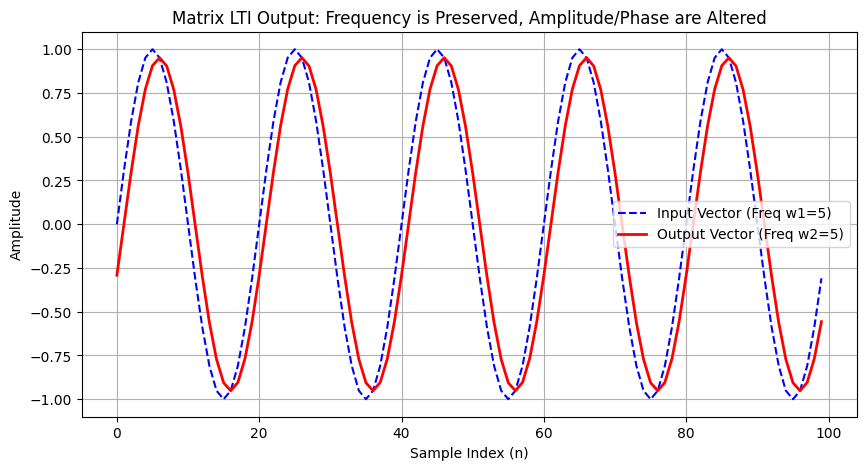
\includegraphics[width=\columnwidth, height=0.8\textheight, keepaspectratio]{download.png}     
\end{frame}


\end{document}
